\documentclass[10pt,a4paper]{article}
\usepackage{graphicx}
\usepackage{subfig}
\usepackage{float}
\usepackage[english]{babel}
\usepackage{hyperref}
\usepackage[font=small,labelfont=bf]{caption}
\textwidth=450pt\oddsidemargin=0pt
\pagenumbering{arabic}

\begin{document}
\begin{titlepage}
\vspace{15mm}
\begin{center}
{\LARGE{\bf Andrea Leganza}}\\
\vspace{3mm}
{\LARGE{\bf MAT. 788513}}\\
\vspace{3mm}
{\LARGE{\bf\ }}\\
\end{center}
\vspace{40mm}
\par
\noindent
\begin{minipage}[t]{0.47\textwidth}
{\large{\bf}}
\end{minipage}
\hfill
\begin{center}
{\large{\bf Final project }}
\end{center}
\vspace{20mm}
\begin{center}
{\large{\bf 12/09/2022}}
\end{center}
\end{titlepage}
\pagebreak


\section{Scene description}
The scene is a diorama of an island placed in the middle of the ocean, the scene can be switched to day and night mode showing/hiding different elements.

\section{Technologies}

The project was developed using Three.js, HTML, CSS and JS

\section{Libraries}

The following libraries were used:

\begin{itemize}
 \item Three.js
 \item Tween.js
 \item dat.gui
\end{itemize}

\section{Assets}

Props were dowloaded from sketchfab.org, cleaed and their topology modified in Blender and then exported in GLTF format:

\begin{itemize}
 \item Castle
 \item Phoenix
 \item Boat
 \item Crab
\end{itemize}

Most of the models required to be cleaned up, their structure and original materials to be modified too. To improve performances the polygons of the models were reduced to quite a 1/10 of the original.

All the animated models were rigged with bones using as a single model  segment so in Blender the models were all splitted as required to accomplish the task to animate "manually" in three.js

Leaves on the water were created using a simple transparent plane and applying on realtime downloaded textures, while fireflies where created using a plane with random color.

\section{User interface}

The GUI was developed using DAT.GUI, the whole interaction is controlled by javascript events. It provides controls to manage mosto of the common interactions aspect of the scene:
 
 \begin{itemize}
 \item Camera: position and rotation
 \item Controls: speed parameters, autorotate parameters
 \item Day/night switch, fog parameters, shadowmap on/off
 \item Ambient light: on/off, intensity and color
 \item Torches: on/off, animation, color, intensity
 \item Spotlight: on/off, shadows, color, intensity, distance, angle, penumbra, position
 \item Sky: on/off
 \item Water: on/off
 \item Particles: night fireflies on/off
 \item Postprocessing: on/off bloom
 \item Audio: on/off, volume
 \item Debug Console Debug: on/off
 \end{itemize}
 
\begin{figure}[H]
\hfill
\subfloat[Menu]{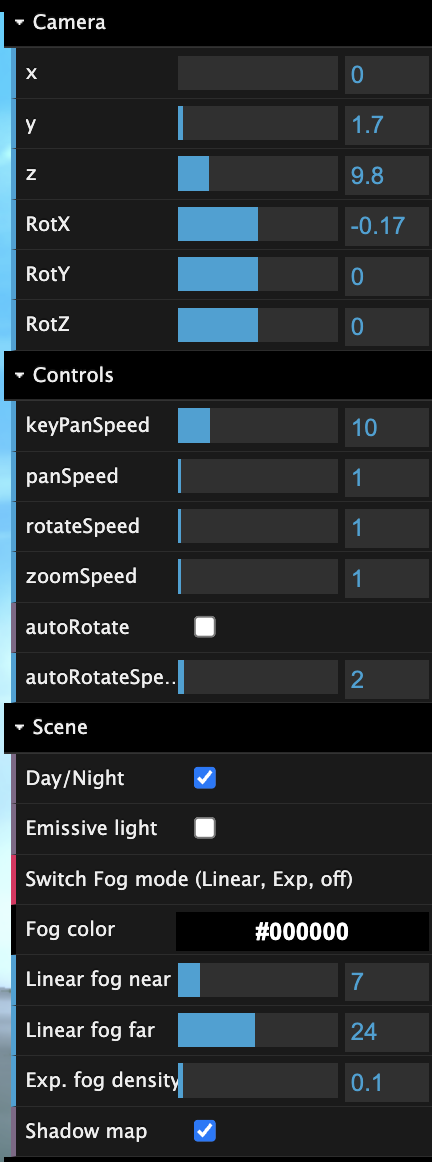
\includegraphics[width=3cm]{ui0}}
\hfill
\subfloat[Menu]{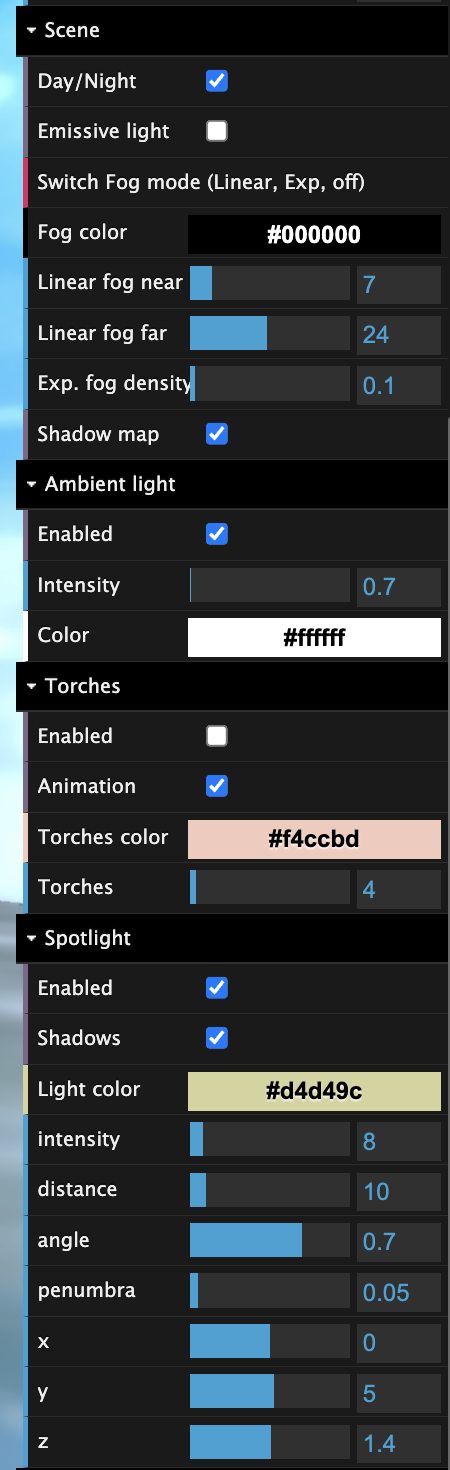
\includegraphics[width=3cm]{ui1}}
\hfill
\subfloat[Menu]{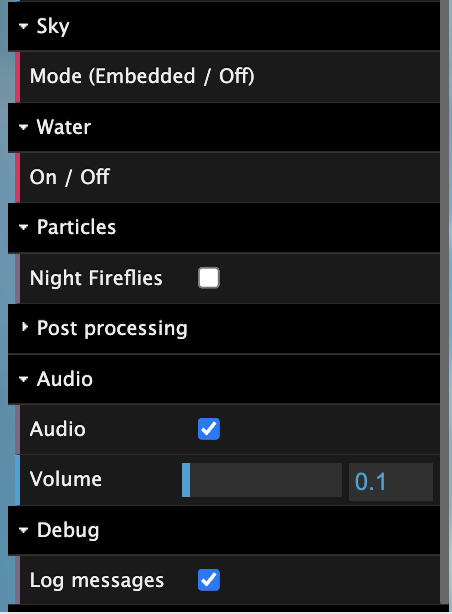
\includegraphics[width=3cm]{ui2}}
\hfill
\caption{Menu views}
\end{figure}


\section{Day/Night mode}

Switching to day/night mode using the GUI button lets to switch to different look of the scene, showing/hiding different elements:

\begin{itemize}
 \item Day: Phoenix flies around  the castle, sky rotates around, leaves float,  water tide
 \item Night: A boat travels around the castle, night sky rotates, fireflies fly around, torches lights up and animate their flame, a crab eat and moves, water tide
\end{itemize}

\begin{itemize}
 \item The sky changes its texture from a cloudy day to a night sky.
 \item Fog changes to exp mode during night to increase the night look darkening the whole scene.
 \item Switching to night/day also customizes the lights with different colors and intensities to improve the scene look.
 \end{itemize}
 
\begin{figure}[H]
\centering
\caption{The DAY mode look using exampke water shader}
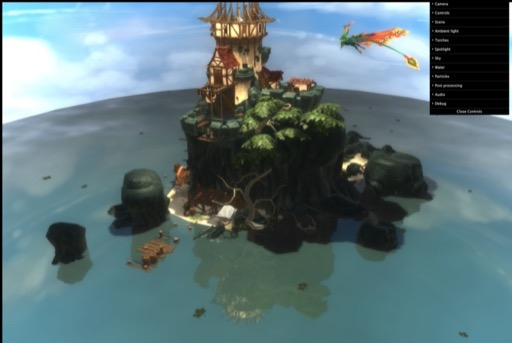
\includegraphics[width=0.9\textwidth,keepaspectratio]{day}
\caption{The NIGTH mode look using example water shader}
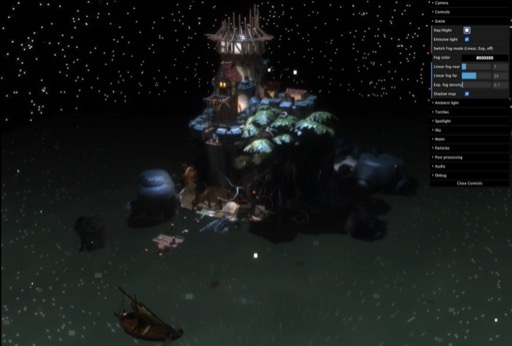
\includegraphics[width=0.9\textwidth,keepaspectratio]{night}
\end{figure}

\begin{figure}[H]
\centering
\caption{The DAY mode look using exampke water shader}
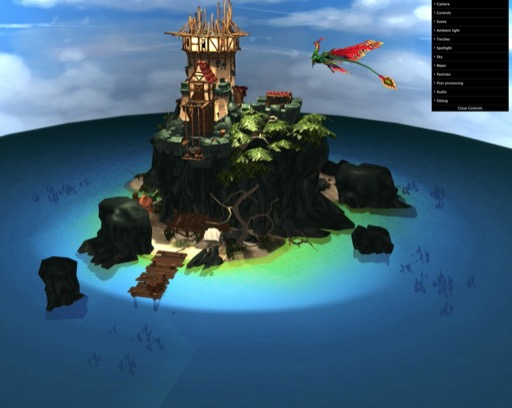
\includegraphics[width=0.8\textwidth,keepaspectratio]{day_sea}
\caption{The NIGTH mode look using example water shader}
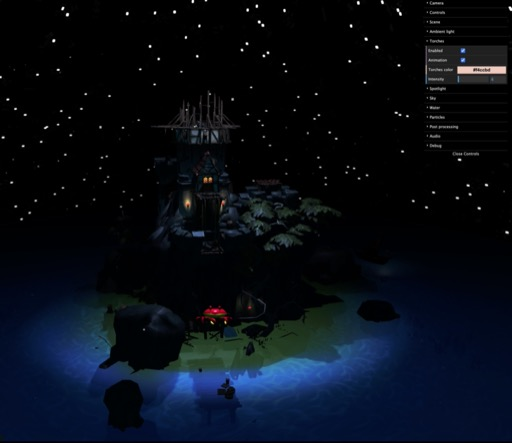
\includegraphics[width=0.8\textwidth,keepaspectratio]{night_sea}
\end{figure}

\section{Sea}

\begin{figure}[H]
\centering
\caption{The model sea}
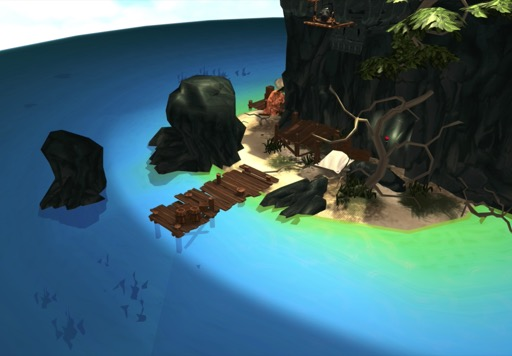
\includegraphics[width=0.8\textwidth]{sea}

\centering
\caption{The THREE.JS/examples sea}
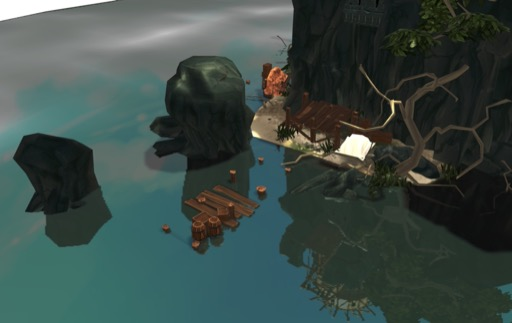
\includegraphics[width=0.8\textwidth]{sea_example}
\end{figure}

\begin{verbatim}
 function animateLiquid(target){

        if (liquidTween!=null){
            TWEEN.remove(liquidTween)
            liquidTween = null
        }

        if (debugMode){
            console.log("Animating water: "+target.name)
        }
        target.position.y = target == water ? -0.1 : 0;

        liquidTween = new TWEEN.Tween(target.position)
            .to({x: 0, 
                 y : target == water ? 0 : 20, 
                 z : 0},
            10000)
            // .delay (1000)
             .yoyo(true)
             .repeat(Infinity)
             .easing(TWEEN.Easing.Quadratic.InOut)
             /*.onUpdate(function () {
               
            })*/
             .start();
    }
\end{verbatim}

\section{Torches}

\begin{figure}[H]
\centering
\caption{One of the torches}
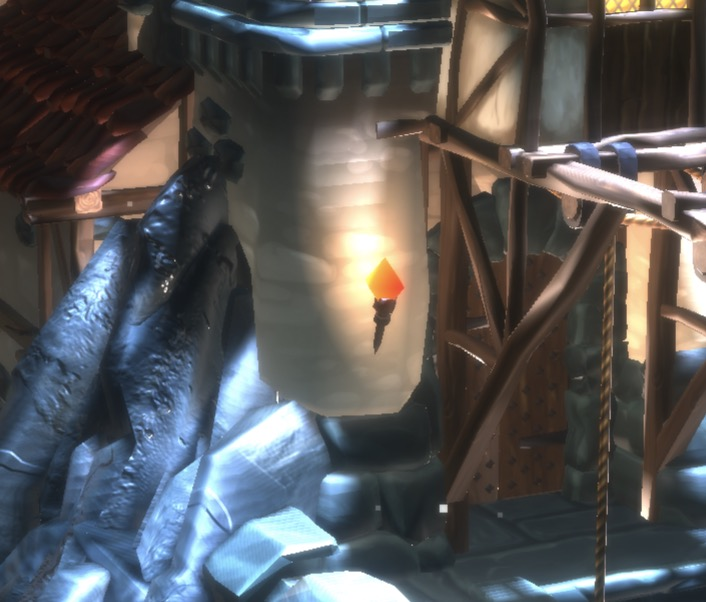
\includegraphics[width=0.8\textwidth]{torch}
\end{figure}


Torches are detected during mesh loading and to them are added:

\begin{itemize}
 \item A spotlight is added with related animation tween
 \item A sphere with some faces to mimic a Platonic solid to simulate the flame
\end{itemize}

To set the color of the flame a custom shader was made, which interpolates between two colors during the time (an uniform updated during the animation loop using a deltatime value) :

\begin{verbatim}
  const sphere = new THREE.SphereGeometry( 3, 4, 2 );

            const mat = new THREE.ShaderMaterial({
                uniforms: {
                    u_time: { type: "f", value: 0 }
                },
                vertexShader: `
                    varying vec2 vUv;
                    uniform float u_time;

                    void main() {
                        vUv = uv;

                        mat4 scale = mat4(vec4(1.0+sin(u_time)*0.1,0.0,0.0,0.0),
                                        vec4(0.0,1.0+sin(u_time)*0.3,0.0,0.0),
                                        vec4(0.0,0.0,1.0+sin(u_time)*0.5,0.0),
                                        vec4(0.0,0.0,0.0,1.0));
                        gl_Position = projectionMatrix * modelViewMatrix * scale * \
                        vec4(position,1.0);
                    }
                `,
                fragmentShader: `
                 uniform float u_time;
                 varying vec2 vUv;
                 void main() {
                  gl_FragColor = vec4(mix(vec3(1,0,0), vec3(1,0.65,0), vUv.y+ \
                  sin(u_time)), 1.0);
                }
            `
            });
\end{verbatim}

\section{Leaves}

Leaves were created with a simple double side transparent plane usig a custom vertex/fragment shader, loading a random local stored leaf texture; they float around the scene with a simple Math.sin movement which starts from a random generated value and the position is updated via the shader position passing the total amount of time elapsed, this approach moves the calculations to the GPU improving performances (istead of updating the mesh.position in the animate loop).

\begin{figure}[H]
\centering
  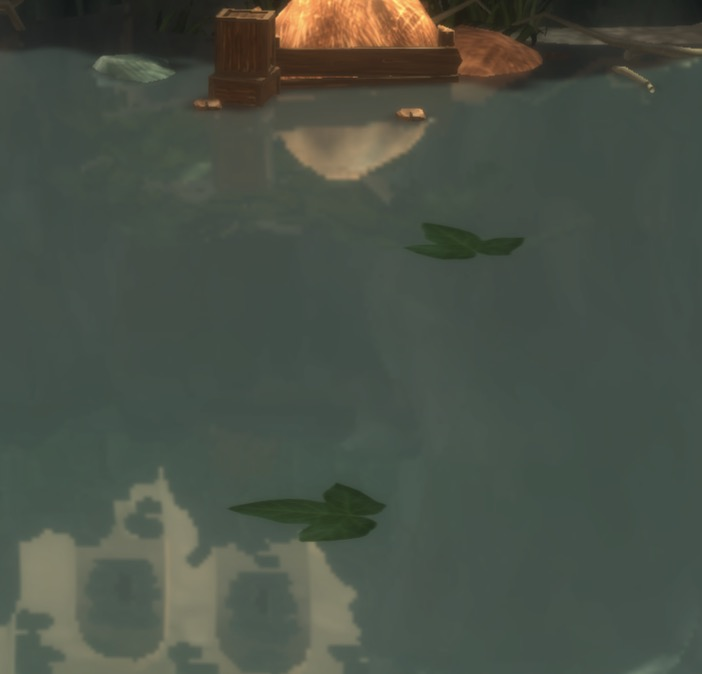
\includegraphics[width=0.5\textwidth]{leaves}
     \caption{The leaves on the surface}
\end{figure}

\begin{verbatim}
     const geometry = new THREE.PlaneGeometry( 1, 1 );
    
        const textureName = 'Textures/leaf'+(Math.floor(Math.random() * 3) + 0)+'.png';

        const texture = new THREE.TextureLoader().load(textureName) ;

        const shaderMat = new THREE.ShaderMaterial({
                uniforms: {
                    u_time: { type: "f", value: 0 },
                    delta: { type: "f", value: 0 },
                    colorTexture: { type: 't', value:texture}
                },
                vertexShader: `
                    varying vec2 vUv;
                    uniform float u_time;
                    uniform float delta;
                    uniform sampler2D colorTexture;

                    void main() {
                        vUv = uv;

                        vec4 newPositon = vec4(sin(delta + u_time)*0.1,0.0,0.0,0.0);

                        gl_Position = (projectionMatrix * modelViewMatrix * vec4(position,1.0)) + newPositon;
                    }
                `,
                fragmentShader: `
                    varying vec2 vUv;
                    uniform sampler2D colorTexture;

                    void main() {
                        vec4 color = texture2D( colorTexture, vUv );
                        gl_FragColor = color * vec4(0.3,0.3,0.3,1.0);
                    }
            `
            });
            shaderMat.side = THREE.DoubleSide
            shaderMat.transparent = true
            shaderMat.depthTest =  true
            shaderMat.depthWrite = false
        
        var leavesCoordPosition = [];

        for (var i= 0; i <30; i++){
            var ranXNum = Math.ceil(Math.random() * 7) * (Math.round(Math.random()) ? 1 : -1)
            var ranYNum = Math.ceil(Math.random() * 7) * (Math.round(Math.random()) ? 1 : -1)

            const pos = new THREE.Vector3(ranXNum,0.01,ranYNum)
            leavesCoordPosition.push(pos);     
        }
    
        leavesCoordPosition.forEach(position => {

            if (debugMode){
                console.log(position);
            }
       
            const mesh = new THREE.Mesh( geometry, shaderMat );

            mesh.rotation.z =  Math.random() * Math.PI * 2; 

            mesh.rotation.x = target == water ? 0 : Math.PI/2;
            
            mesh.position.set(  position.x*(target == water ? 1 : 100),
                                position.y,
                                position.z*(target == water ? 1 : 100));
            
            let s = Math.random() *(target == water ? 0.1 : 30) + 0.1;
            mesh.scale.set(s, s, s);
            mesh.userData.delta = Math.random() * Math.PI * 2;
            mesh.material.uniforms["delta"].value = mesh.userData.delta

            floatingObjects.push(mesh);
        
            target.add(mesh);
        });
\end{verbatim}

\section{Fireflies}

Fireflies were developed as simple squares of different sizes and colors embbeded inside a BufferGeometry with a PointsMaterial, thei change color during the render loop.

\begin{figure}[H]
 \centering
  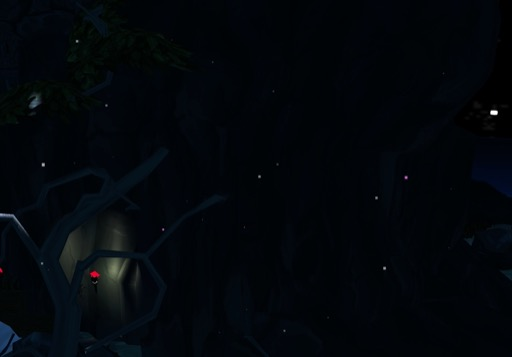
\includegraphics[width=0.6\textwidth]{fireflies}
     \caption{Fireflies flying around the night scene}
\end{figure}

\begin{verbatim}

function placeFireFlies(){
  particleMode = ParticleMode.on
        
        if (particlestGroup != null){

            particlestGroup.visible = true

            return
        }

        particlestGroup = new THREE.Group();

        const geometry = new THREE.BufferGeometry();
        const vertices = [];

        const textureLoader = new THREE.TextureLoader();

        const sprite = textureLoader.load( '' );

        for ( let i = 0; i < 100; i ++ ) {

            const x = Math.random() * 9 - 4.5;
            const y = Math.random() * 9 - 4.5;
            const z = Math.random() * 9 - 4.5;

            vertices.push( x, y, z );
        }

        geometry.setAttribute( 'position', new THREE.Float32BufferAttribute( vertices, 3 ) );

        particleParameters = [
            [[ 1.0, 1.0, 1.0 ], sprite, 0.05 ],
            [[ 0.86, 0.86, 0.67], sprite, 0.02],
            [[ 0.3, 0.3, 0.3], sprite, 0.03 ],
        ];

        for ( let i = 0; i < particleParameters.length; i ++ ) {

            const color = particleParameters[ i ][ 0 ];
            const sprite = particleParameters[ i ][ 1 ];
            const size = particleParameters[ i ][ 2 ];

            particleMaterials[ i ] = new THREE.PointsMaterial( { size: size, blending:
             THREE.AdditiveBlending, depthTest: false, transparent: true } );
            particleMaterials[ i ].color.setHSL( color[ 0 ], color[ 1 ], color[ 2 ] );

            const particles = new THREE.Points( geometry, particleMaterials[ i ] );

            particlesEffects.push(particles);

            particlestGroup.add( particles );
        }

        scene.add(particlestGroup)
\end{verbatim}


\section{Animations}

Animations were implemented with different techniques:

\begin{itemize}
 \item Updating rotation/position properties of mesh directly in the render loop
 \item Updating UV offset
 \item Using Tween.JS
 \item Updating shader properties
\end{itemize}

\bigbreak
\bigskip

The following elements were animated:
\begin{itemize}
 \item Sky: rotates on z axis on day, on z and y axis during night (using uv offset)
 \item Water: translates up/down to simulate low/high tide with an easing
 \item Torches: flame scales and rotates, their light glows randomly
 \item Leaves on the water: oscillate on the surface and float vertically
 \item Phoenix (day mode) flies and rotate around a spline (CatmullRomCurve3)
 \item Boat (night mode) rotate around castle and floats up/down
 \item Boat lantern (night mode): oscillates during boat movement
 \item Crab (night mnode): every leg moves, claws move, crab moves left/right, crab lookA the camera
 \item Fireflies particles: randomly move and change colors
 \end{itemize}

\section{Phoenix}

The original model was rigged and was a sigle mesh, the first operation that was done on it was to remove the whole rigging hierarchy and split the different segments in Blender, then a proper hierarchy was created starting  from the body. To speed up the animation process "custom properties" were  added to each of the mesh segments to pass axis, easing, delay and movement direction which were read in three.js by accessing the userdata property; these properties were then used by Tween.js to animate as needed. All the meshes required to set an ad hoc pivot to be properly aimated.

\begin{figure}[H]
   \caption{The phoenix structure}
  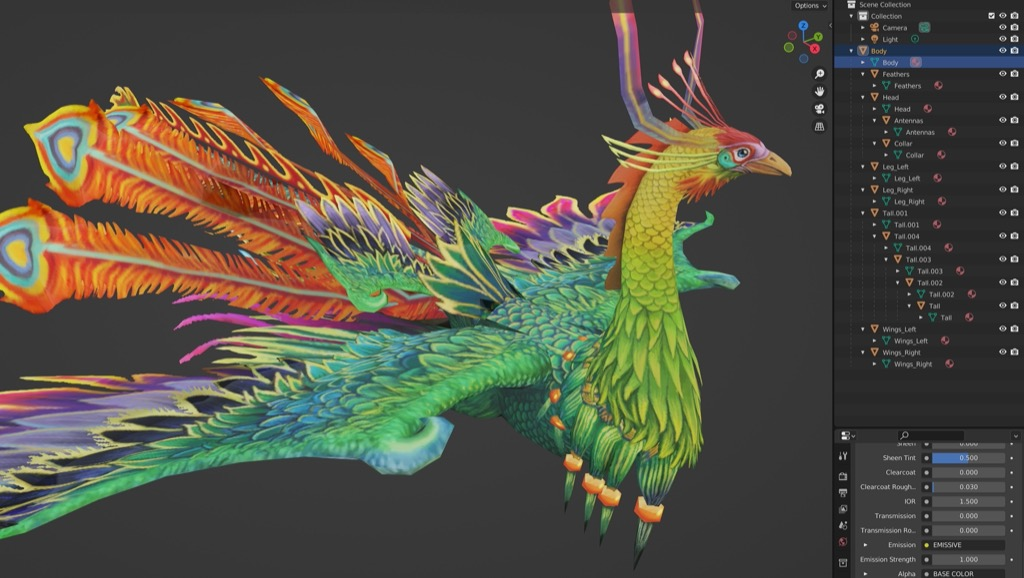
\includegraphics[width=1\textwidth]{phoenix}
\end{figure}

\begin{figure}[H]
\caption{Custom properties used to pass data to Three.js}
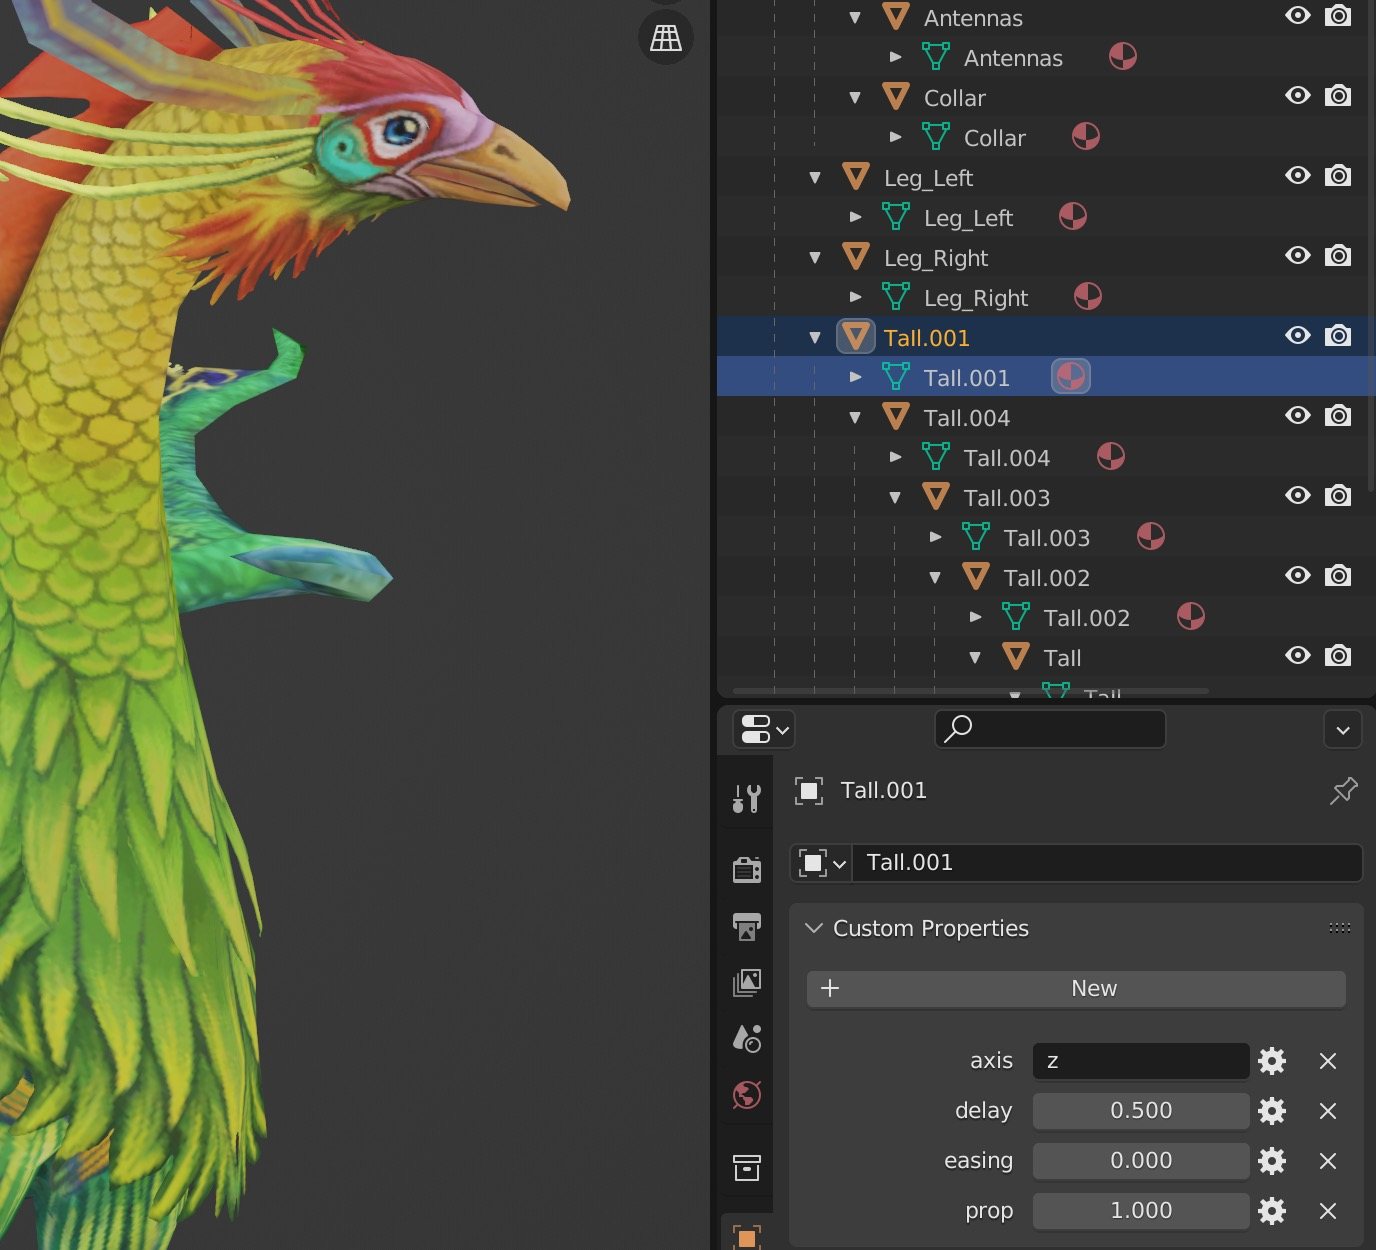
\includegraphics[width=1\textwidth]{phoenix_data}
\end{figure}

\section{Boat}

The boat was cleaned up, the pivot was changed to a proper position, the lantern was separated from the boat and the pivot set in the correct position for both of them to proper support the animation process.

\begin{center}
\begin{figure}[H]
\caption{The boat structure}
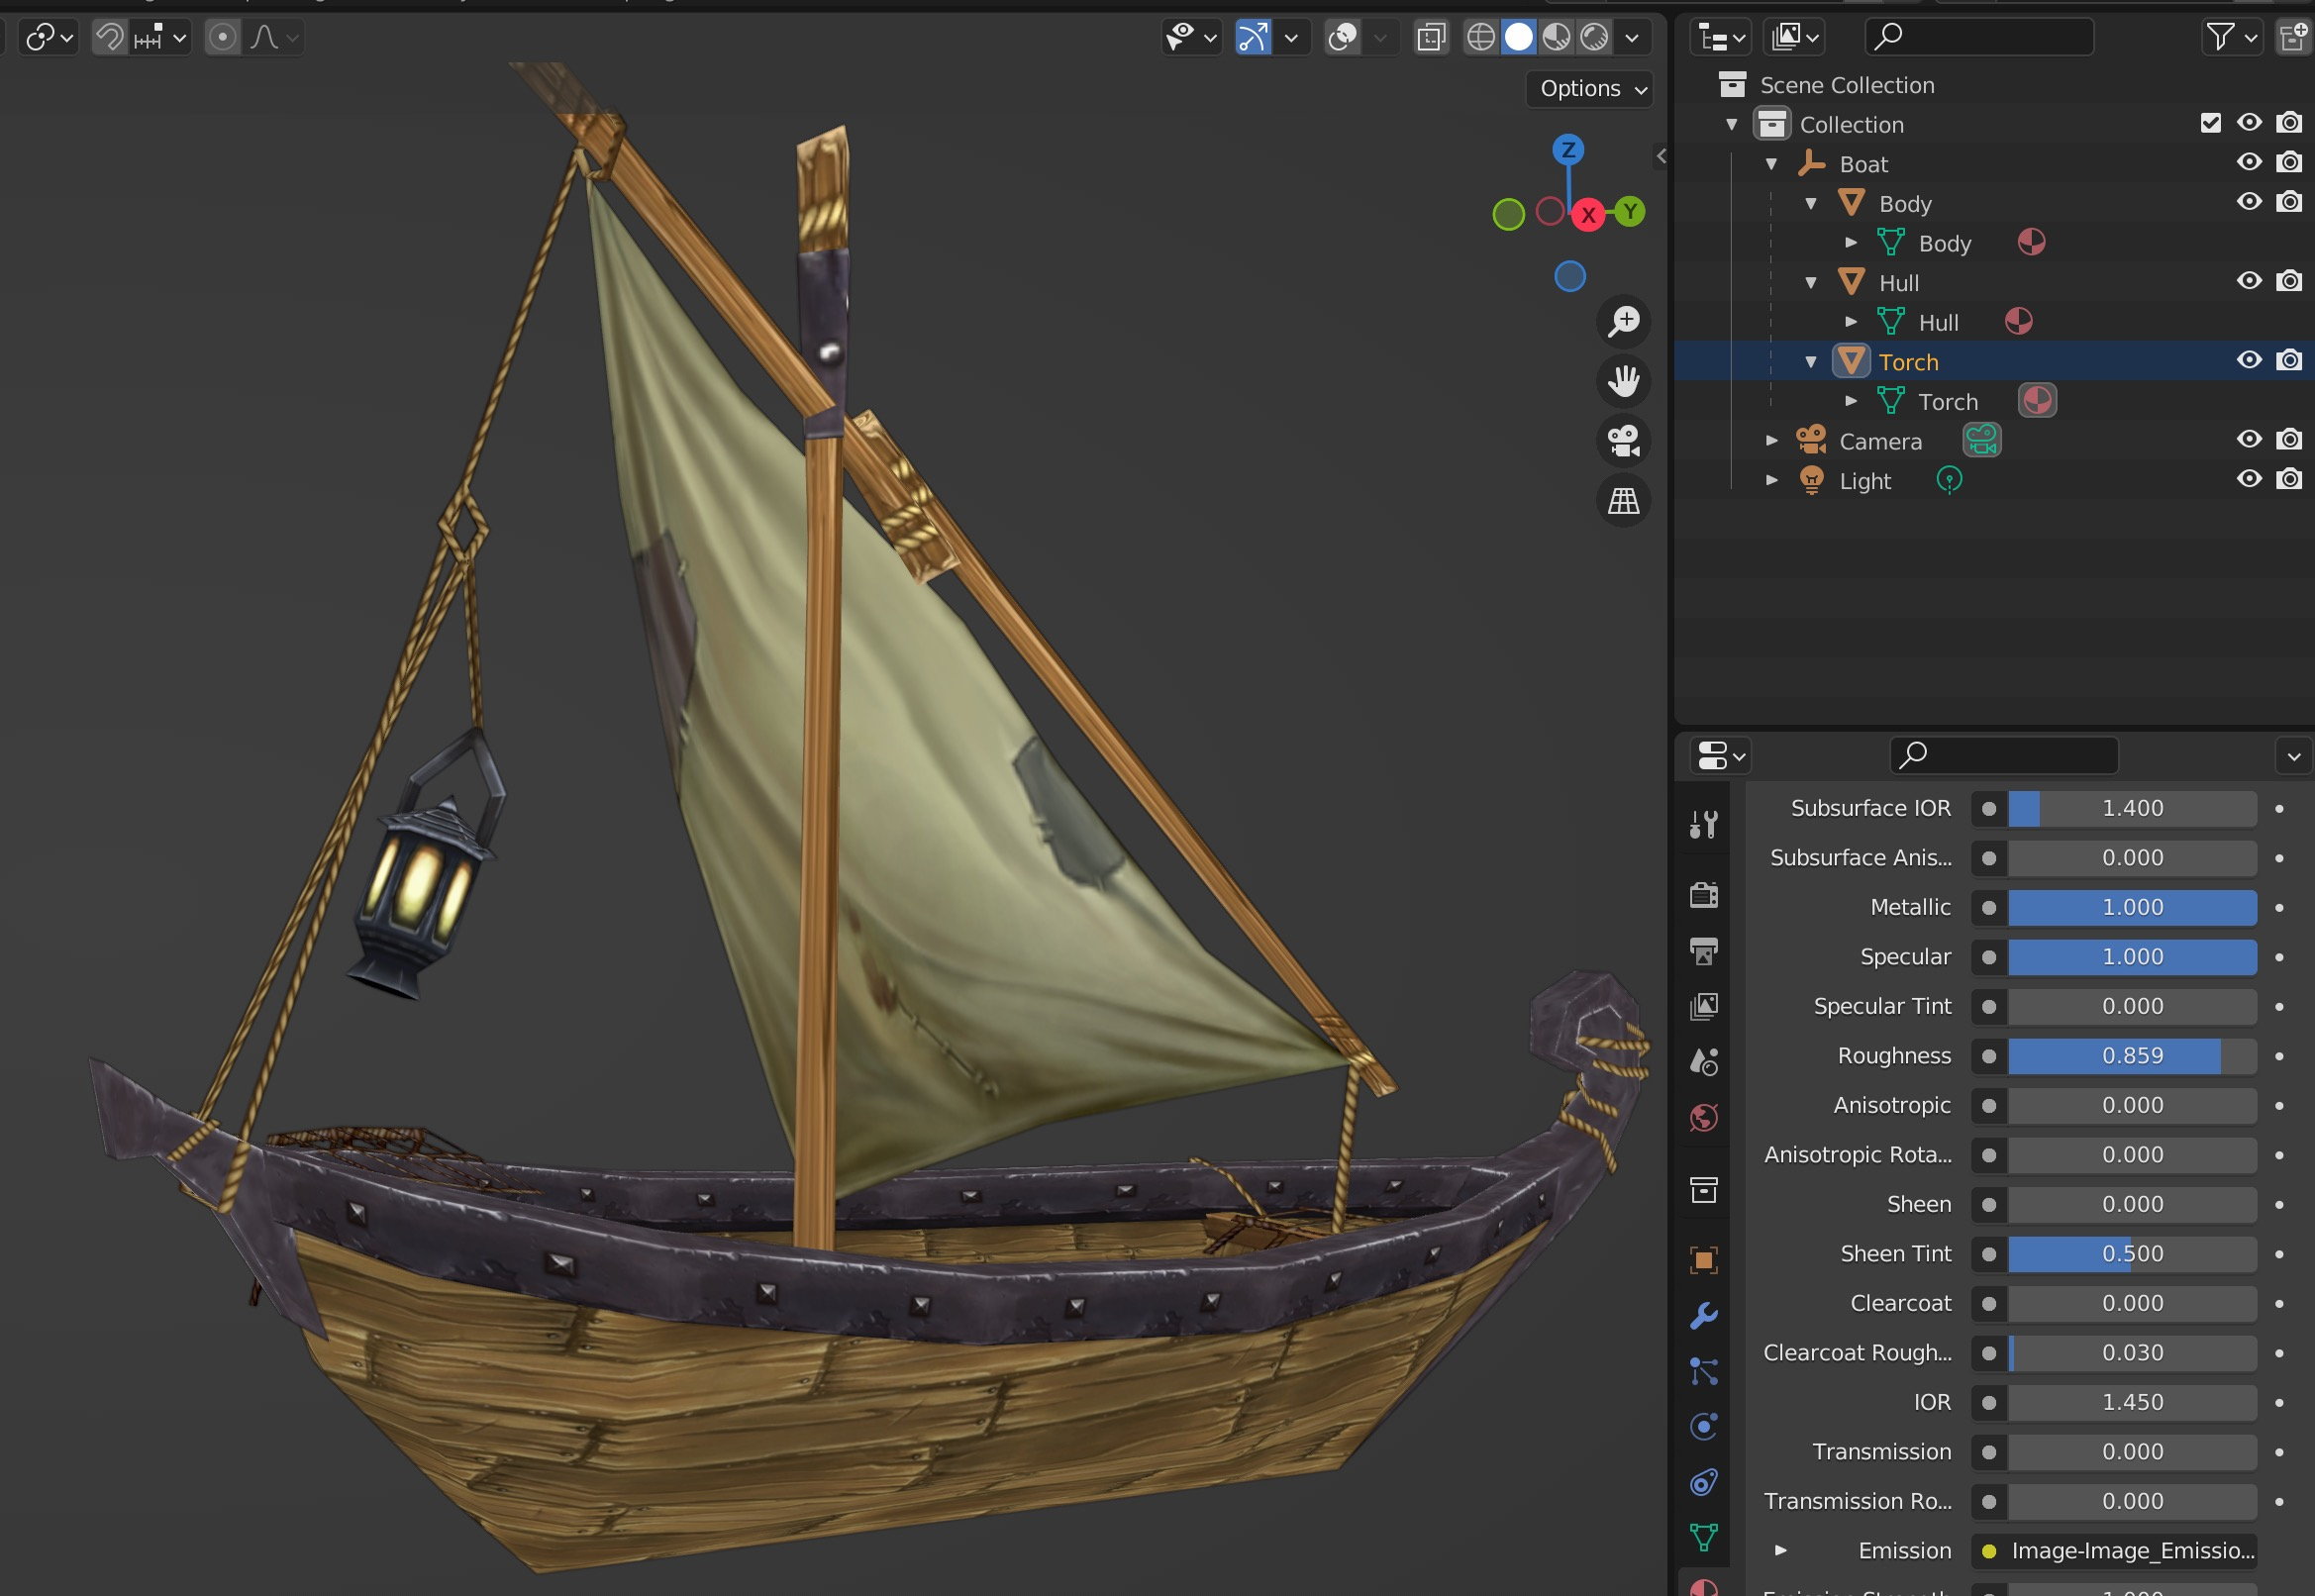
\includegraphics[width=1\textwidth]{boat}
\end{figure}
\end{center}


\section{Crab}

The crab was cleaned up, the mesh was ann unique geometry, so it was splitted in segments and its poly counts  wasreduced using Blender modifier; all the pivots were changed to match a proper position; crab legs are animated using Tween.js using the same approach of the Phoenix so using model passed custom properties. The crab updates it's rotation using the mesh.lookAt(camera.position) so always lookig towards the user.

\begin{center}
\begin{figure}[H]
\caption{The crab structure}
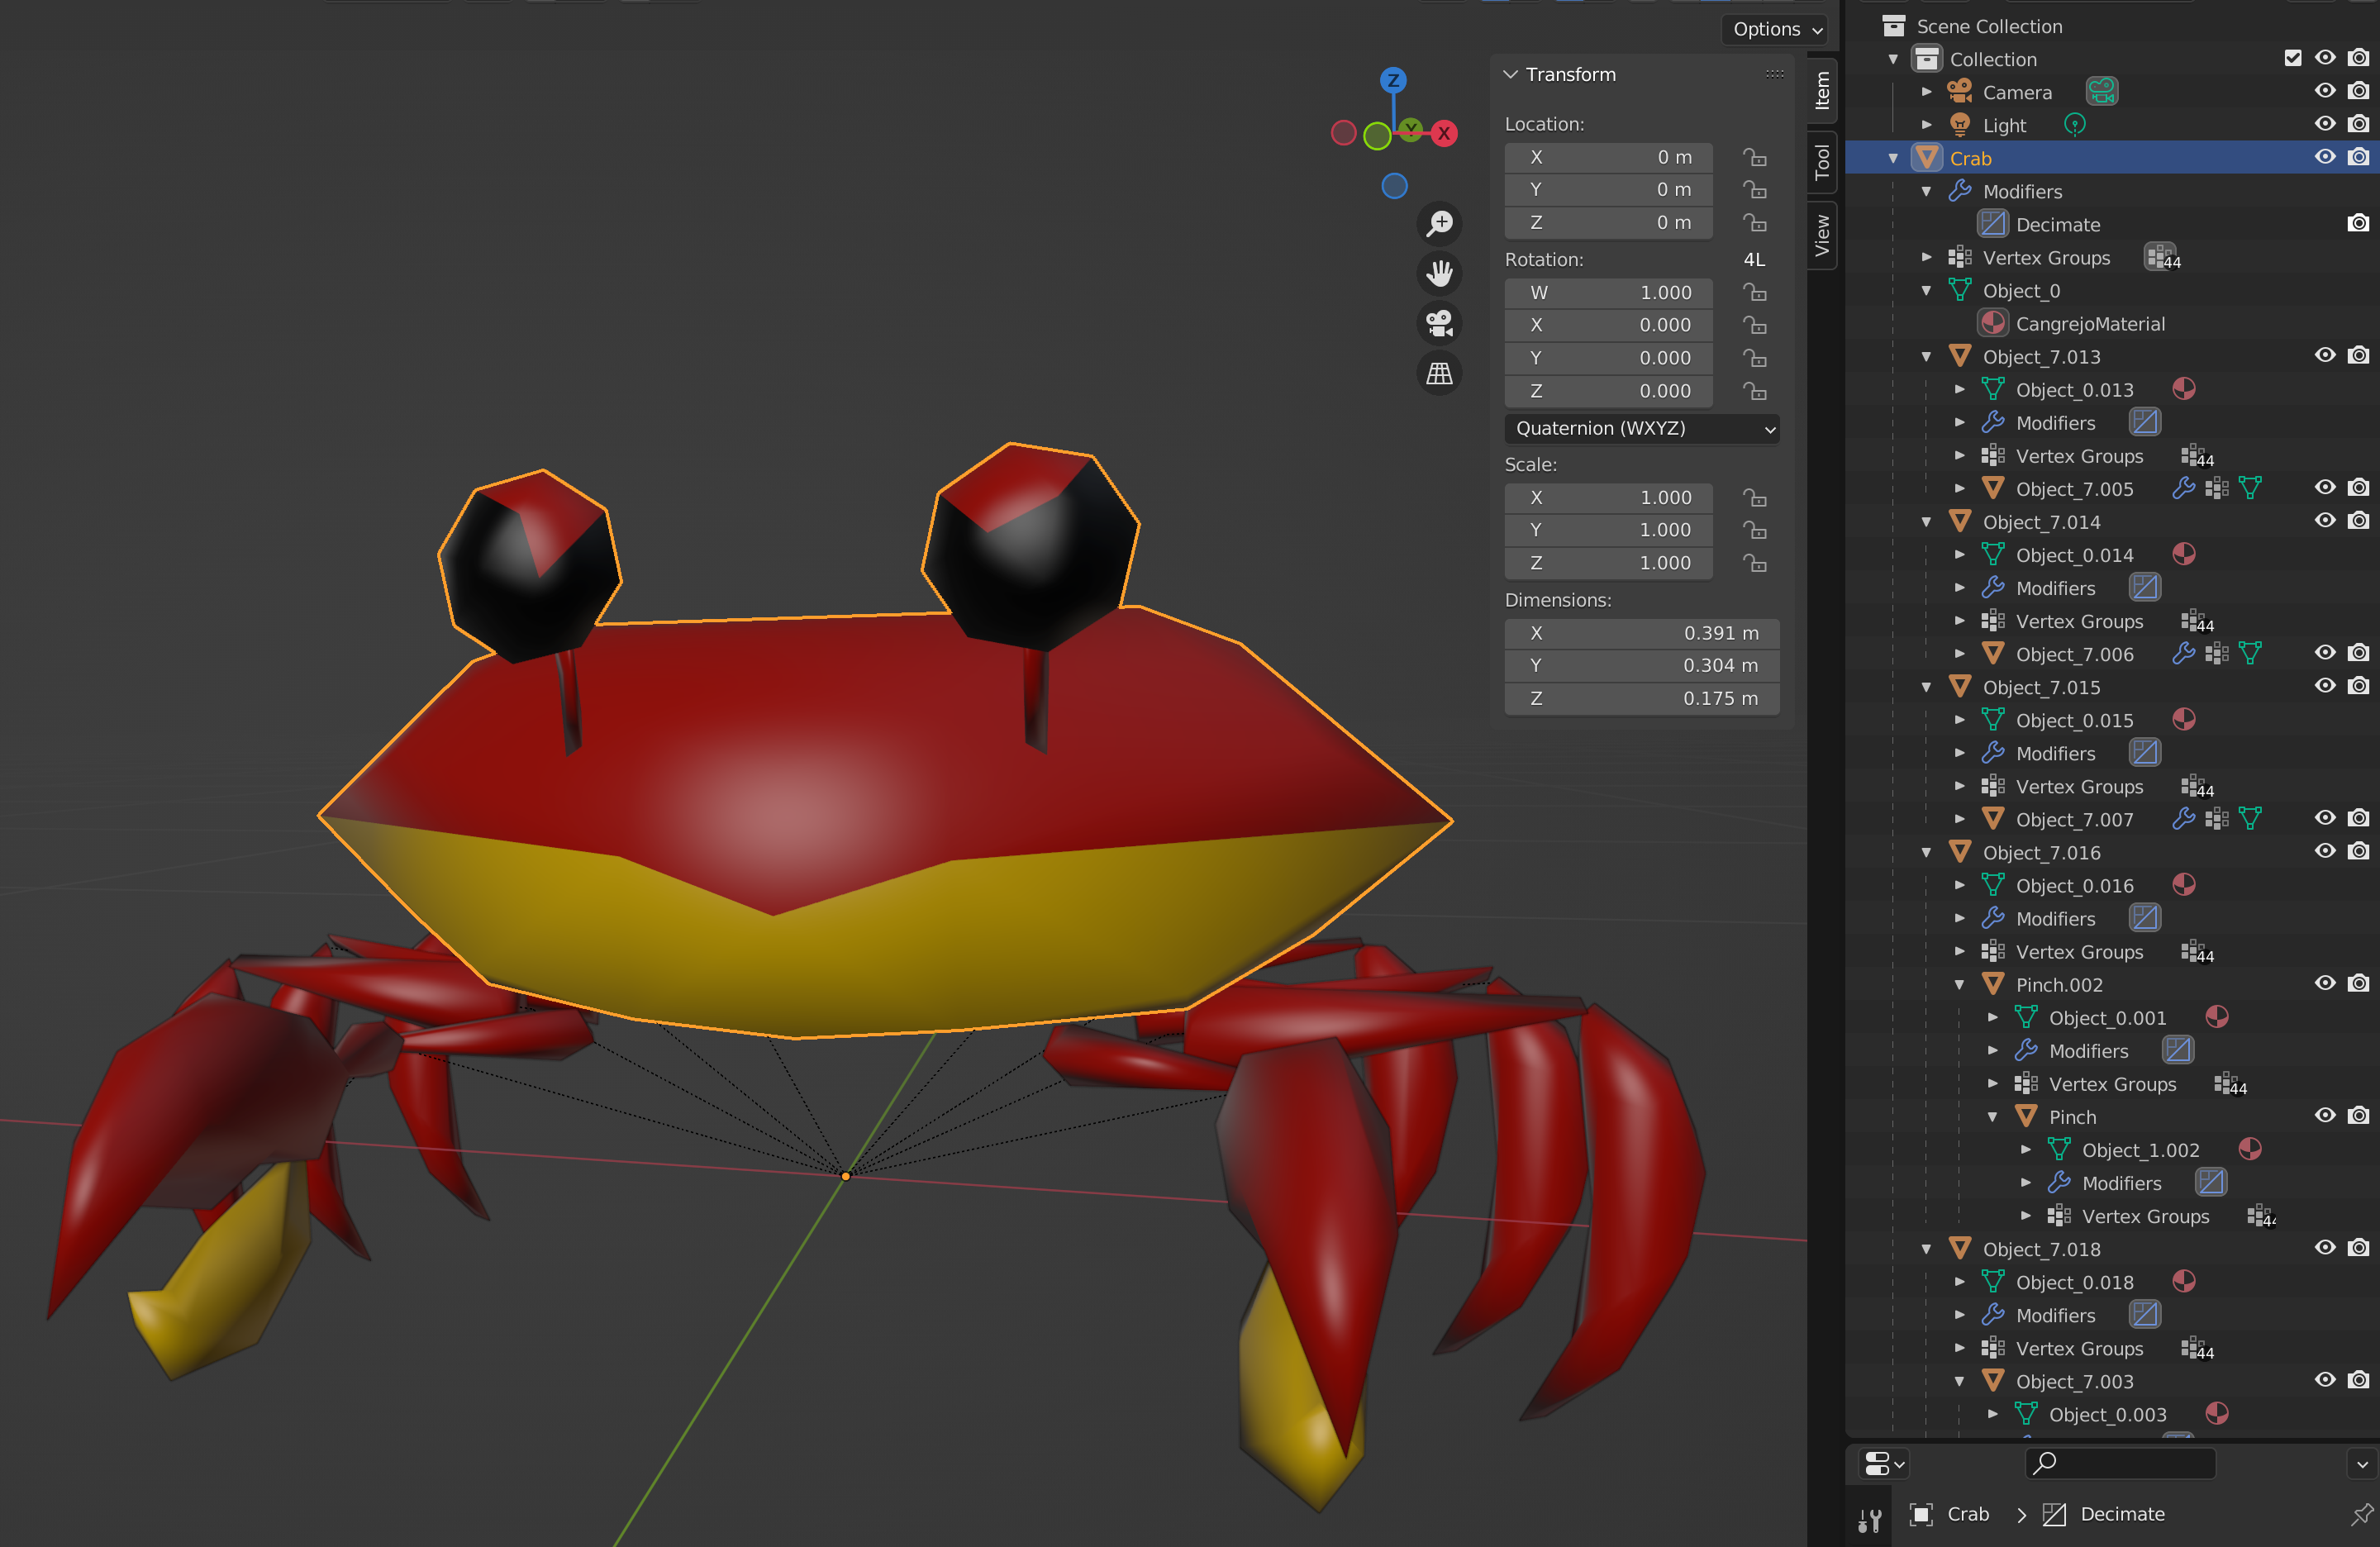
\includegraphics[width=1\textwidth]{crab}
\end{figure}
\end{center}

\begin{verbatim}
function animateCrabMesh(mesh, axis, delta, delay, easing, speed = 1){

if (debugMode){
    console.log("Animating crab: "+mesh.name);
}

const tween = new TWEEN.Tween(mesh.rotation)
    .to({[axis]:mesh.rotation[axis] + 0.2*delta},1000*speed)
    .yoyo(true)
    .delay(delay != null ? delay*1000 : 0)
    .repeat(Infinity)
    .easing(easing != null ? (easing == 1 ? TWEEN.Easing.Linear.None : TWEEN.Easing.Quadratic.InOut) : TWEEN.Easing.Linear.None)
    .start()

    crabTweens.push(tween)

}
\end{verbatim}

\section{Textures}
The following textures were used:

\begin{itemize}
\item Base/Albedo map
\item Normal map
\item Emissive map
\end{itemize}

For some models the normal map was generated from base/albedo map using an online service (\url{https://cpetry.github.io/NormalMap-Online/}); for emission some maps were generated by hand modifying in Krita the base map removing opaque areas; the emissive intensity effect was increased during the load of the models and a GUI option is available to change this value.

\section{Lights}
The lights used in the scene were:

\begin{itemize}
\item An Ambient Light to light the whole scene
\item A Spotlight to light from the top the castle
\item Four point lights for each torch lights to simulate the light of the torches
\item A spot light on the boat
\end{itemize}

\section{Audio}

A seashore audio loop sound effect is provided, during the day mode a seagull sound is played too, while during the night a crickets soud is played.

\section{Render loop}

\begin{verbatim}
 function animate() {

        if (loading){
            return
        }

        deltaTime = clock.getDelta();
     
        totalTime+=deltaTime;

        if (skyEmbedded!=null && skyEmbedded.visible) {

            if(skyTime == SkyTime.day) {
                skyEmbedded.material.map.offset.x -= 0.001*deltaTime; 
            }
            else {
                skyEmbedded.material.map.offset.x -= 0.001*deltaTime; 
                skyEmbedded.material.map.offset.y += 0.001*deltaTime; 
            }
        }
        
        if (waterUniforms!=null && water!=null) {
            waterUniforms[ 'time' ].value += 0.1*deltaTime;
        }

        if (boatGroup!=null) {
            if (boatGroup.parent == water){
                boatGroup.rotation.y += 0.02*deltaTime;
                boatGroup.position.z = Math.cos(totalTime)*0.05;
            }
            else if (boatGroup.parent==sea) {
             boatGroup.rotation.y += 0.02*deltaTime;
             boatGroup.position.z = Math.cos(totalTime)*0.05;
            } 
        }

        //Fireflies
        if (particlestGroup != null && particlestGroup.visible){

            const time = Date.now() * 0.00001;
            
            for ( let i = 0; i < particlesEffects.length; i ++ ) {
                particlesEffects[i].rotation.y = time * ( i < 4 ? i + 1 : - ( i + 1 ) );
            }

            for ( let i = 0; i < particleMaterials.length; i ++ ) {
                const color = particleParameters[ i ][ 0 ];
                const h = ( 360 * ( color[ 0 ] + time ) % 360 ) / 360;
                particleMaterials[ i ].color.setHSL( h, color[ 1 ], color[ 2 ] );

            }
        }

        //Torchlights  animation
        for (const torch of torchLights){
            if (torch.light.visible){
                torch.mesh.material.uniforms["u_time"].value += deltaTime;
            }
        }
       
        //Phoenix animation
        if (phoenix!=null) {
            movePhoenixAroundPath(deltaTime*0.05);
        }

        //Leaves animation
        floatingObjects.forEach(obj => {
            obj.material.uniforms["u_time"].value = totalTime
            //obj.position.y+= Math.sin(obj.userData.delta + totalTime) * 0.001;
        });

        //Crab
        if (crab!=null)
        crab.lookAt(camera.position)

        requestAnimationFrame( animate );
        !postProcessingMode ? renderer.render( scene, camera ) : \
         postProcessing.composer.render(deltaTime);
        TWEEN.update();

        stats.update()
    }
\end{verbatim}

\section{Notes}

The performances during camera look aren't great, performances should be improved: using lightmapping, storing shadows and reducing polygon count, also moving most of  the animations to  the shaders will improve the  whole experience reducing render time. An alternative version of the water is provided enabling the proper option available under the "sea" menu voice (the sea is took from examples folder).

\bigbreak
\bigbreak
Andrea Leganza - 788513

\end{document}

